%%%%%%%%%%%%%%%%%%%%%%%%%%%%%%%%%%%%%%%%%%%%%%%%%%%%%%%%%%%%%%%%%%%%%%%%%%%%%%%%%%%
%% This project aims to create the UFC template for presentation.                %%
%% author: Maurício Moreira Neto - Doctoral student in Computer Science (MDCC)   %%
%% contacts:                                                                     %%
%%    e-mail: maumneto@ufc.br                                                    %%
%%    linktree: https://linktr.ee/maumneto                                       %%
%%%%%%%%%%%%%%%%%%%%%%%%%%%%%%%%%%%%%%%%%%%%%%%%%%%%%%%%%%%%%%%%%%%%%%%%%%%%%%%%%%%
\documentclass{libs/ufc_format}
% Inserting the preamble file with the packages
%%%%%%%%%%%%%%%%%%%%%%%%%%%%%%%%%%%%%%%%%%%%%%%%%%%%%%%%%%%%%%%%%%%%%
%% This file contains the packages that can be used in the beamer. %%
%%%%%%%%%%%%%%%%%%%%%%%%%%%%%%%%%%%%%%%%%%%%%%%%%%%%%%%%%%%%%%%%%%%%%
% Package to fonts family
\usepackage[T1]{fontenc}
% Package to accentuation
\usepackage[utf8]{inputenc}
% Package to Portuguese language
\usepackage[brazil]{babel}
% Package to Figures
\usepackage{graphicx}
% Package to the colors
\usepackage{color}
% Package to the colors
\usepackage{xcolor}
% Packages to math symbols and expressions
\usepackage{amsfonts, amssymb, amsmath}
% Package to multiple lines and columns in table
\usepackage{multirow, array} 
% Package to create pseudo-code
% For more detail of this package: http://linorg.usp.br/CTAN/macros/latex/contrib/algorithm2e/doc/algorithm2e.pdf
\usepackage{algorithm2e}
% Package to insert code
\usepackage{listings} 
\usepackage{keyval}
% Package to justify text
\usepackage[document]{ragged2e}
% Package to manage the bibliography
\usepackage[backend=biber, style=numeric, sorting=none]{biblatex}
% Package to facilities quotations
\usepackage{csquotes}
% Package to use multicols
\usepackage{multicol}

% Packages added by me
\usepackage{url}
\usepackage{tikz}
%\usepackage{multimedia}
%\usepackage{media9}[playbutton=plain, windowed=1280x720]
% Inserting the references file
\bibliography{references.bib}
\renewcommand*{\bibfont}{\scriptsize}

% Title
\title[ML]{\huge\textbf{Machine Learning}}
% Subtitle
\subtitle{Parte 3}
% Author of the presentation
\author{Evandro J.R. Silva}
% Institute's Name
\institute[Estácio Teresina]{
    % email for contact
    \normalsize{\email{ejrs.profissional@gmail.com}}
    \newline
    % Department Name
    \department{Bacharelado em Ciência da Computação}
    \newline
    % university name
    %\ufc
    \estaciothe
}
% date of the presentation
\date{\today}


%%%%%%%%%%%%%%%%%%%%%%%%%%%%%%%%%%%%%%%%%%%%%%%%%%%%%%%%%%%%%%%%%%%%%%%%%%%%%%%%%%
%% Start Document of the Presentation                                           %%               
%%%%%%%%%%%%%%%%%%%%%%%%%%%%%%%%%%%%%%%%%%%%%%%%%%%%%%%%%%%%%%%%%%%%%%%%%%%%%%%%%%
\begin{document}
% insert the code style
%%%%%%%%%%%%%%%%%%%%%%%%%%%%%%%%%%%%%%%%%%%%%%%%%%%%%%%%%%%%%%%%%%%%%%%%%%%%%%%%%%%
%% This file contains the style of the codes show in slides.                     %%
%% The package used is listings, but it possible to used others.                 %%
%%%%%%%%%%%%%%%%%%%%%%%%%%%%%%%%%%%%%%%%%%%%%%%%%%%%%%%%%%%%%%%%%%%%%%%%%%%%%%%%%%%

% color used in the code style
\definecolor{codegreen}{rgb}{0,0.6,0}
\definecolor{codegray}{rgb}{0.5,0.5,0.5}
\definecolor{codepurple}{rgb}{0.58,0,0.82}
\definecolor{codebackground}{rgb}{0.95,0.95,0.92}

% style of the code!
\lstdefinestyle{codestyle}{
    backgroundcolor=\color{codebackground},   
    commentstyle=\color{codegreen},
    keywordstyle=\color{magenta},
    numberstyle=\tiny\color{codegray},
    stringstyle=\color{codepurple},
    basicstyle=\ttfamily\footnotesize,
    frame=single,
    breakatwhitespace=false,         
    breaklines=true,                 
    captionpos=b,                    
    keepspaces=true,                 
    numbers=left,                    
    numbersep=5pt,                  
    showspaces=false,                
    showstringspaces=false,
    showtabs=false,                  
    tabsize=2,
    title=\lstname 
}

\lstset{style=codestyle}


%% ---------------------------------------------------------------------------
% First frame (with tile, subtitle, ...)
\begin{frame}{}
    \maketitle
\end{frame}

%% ---------------------------------------------------------------------------
% Second frame
\begin{frame}{Sumário}
    \begin{multicols}{2}
        \tableofcontents
    \end{multicols}
\end{frame}

%=============================================================================
% SECTION 1
%=============================================================================
\section{Principais Algoritmos}

\begin{frame}{}
    \centering
    \LARGE
    Principais Algoritmos
\end{frame}

\begin{frame}{Principais Algoritmos}
    \begin{itemize}
        \item Aprendizado Supervisionado
            \begin{itemize}
                \item Classificação
                    \begin{itemize}
                        \item Naive Bayes
                        \item k-NN
                        \item Árvore de Decisão
                        \item \alert{Redes Neurais Artificiais}
                    \end{itemize}
                \item Regressão
                    \begin{itemize}
                        \item Regressão Logística
                    \end{itemize}
            \end{itemize}
        \item Aprendizado Não Supervisionado
            \begin{itemize}
                \item k-Means
            \end{itemize}
    \end{itemize}
\end{frame}

%=============================================================================
% SECTION 2
%=============================================================================
\section{Redes Neurais Artificiais}

\begin{frame}{}
    \centering
    \LARGE
    Aprendizado Supervisionado\\
    \vspace{0.5cm}
    \LARGE
    Classificação\\
    \vspace{0.5cm}
    \Large
    Redes Neurais Artificiais
\end{frame}

\begin{frame}{Redes Neurais Artificiais}
    \begin{block}{O que são Redes Neurais Artificiais?}
        \justifying
        "Redes Neurais Artificiais (RNAs) são sistemas paralelos distribuídos compostos por unidades de processamento simples (nodos) que calculam determinadas funções matemáticas (normalmente não-lineares). Tais unidades são dispostas em uma ou mais camadas interligadas por um grande número de conexões, geralmente unidirecionais. Na maioria dos modelos estas conexões estão associadas a pesoas, os quais armazenam o conhecimento representado no modelo e servem para ponderar a entrada recebida por cada neurônio da rede. O funcionamento destas redes é inspirado em uma estrutura física concebida pela natureza: o cérebro humano." \cite{blc00}
    \end{block}
\end{frame}

\begin{frame}{Redes Neurais Artificiais}
    \begin{itemize}
        \justifying
        \item Existem vários tipos de RNAs, e vamos ver duas básicas e comuns: Perceptron e MLP (\textit{Multi Layer Perceptron}).
        \item<2-> Não veremos as outras por questão de tempo e também porque estamos em um minicurso introdutório.
    \end{itemize}
\end{frame}

%-----------------------------------------------------------------------------
% SUBSECTION 2.1
%-----------------------------------------------------------------------------
\subsection{Perceptron}

\begin{frame}{Redes Neurais Artificiais}
    \begin{itemize}
        \item Perceptron
            \begin{itemize}
                \justifying
                \item O Perceptron consiste em apenas um único neurônio artificial, o qual recebe várias entradas, é capaz de processá-las e retorna uma saída.\\
                \uncover<2->{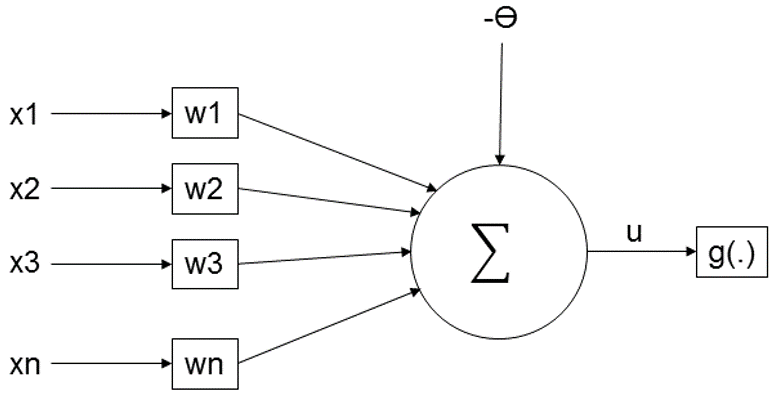
\includegraphics[scale=0.5]{media/neuronio}}
                    \begin{itemize}
                        \item<3-> Sinais de entrada: $\{x_{1}, x_{2}, x_{3}, ..., x_{n}\}$;
                        \item<4-> Pesos sinápticos: $\{w_{1}, w_{2}, w_{3}, ..., w_{n}\}$;
                        \item<5-> Combinador linear: $\Sigma$;
                        \item<6-> Limiar de ativação: $\theta$;
                        \item<7-> Potencial de ativação: $u = \sum\limits^{n}_{i=1}w_{i}\cdot x_{i} - \theta$;
                        \item<8-> Função de ativação: $g(.)$;
                        \item<9> Sinal de saída: $y = g(u)$;
                    \end{itemize}
            \end{itemize}
    \end{itemize}
\end{frame}

\begin{frame}{Redes Neurais Artificiais}
    \begin{itemize}
        \item Perceptron
            \begin{itemize}
                \item Funcionamento básico:
                    \begin{enumerate}
                        \justifying
                        \item<2-> Cada entrada é um valor. Multiplique cada entrada pelo peso correspondente;
                        \item<3-> Faça a combinação de todas as entradas (já multiplicadas com os pesos) com o limiar de ativação. A combinação é a soma de todos os valores.
                        \item<4-> Execute a função de ativação. Essa função tem como entrada a combinação das entradas e limiar de ativação. A partir do valor recebido a função vai retornar outro valor. Por exemplo: se o valor for $\ge 0$ a função retorna 1, senão, retorna 0. O retorno dessa função é justamente a saída $y$.
                        \item<5> Se o aprendizado for supervisionado e a saída estiver errada, ajuste os pesos de acordo com alguma função escolhida.
                    \end{enumerate}
            \end{itemize}
    \end{itemize}
\end{frame}

\begin{frame}{Redes Neurais Artificiais}
    \begin{itemize}
        \item Perceptron\\
        \begin{exampleblock}{Exemplo}
            \begin{itemize}
                \justifying
                \item Dada uma rede do tipo Perceptron formada por um neurônio com três terminais de entrada, utilizado os pesos iniciais $w_{0} = 0,4$, $w_{1} = -0,6$ e $w_{2} = 0,6$, limiar $\theta = 0,5$ e uma taxa de aprendizado $\eta = 0,4$. Responda os itens abaixo:
                    \begin{enumerate}
                        \justifying
                        \item Ensinar a rede a gerar a saída -1 para o padrão 001 e a saída +1 para o padrão 110;
                        \item A que classe pertencem os padrões 111, 000, 100, 011?
                    \end{enumerate}
            \end{itemize}
        \end{exampleblock}
    \end{itemize}
\end{frame}

\begin{frame}{Redes Neurais Artificiais}
    \begin{itemize}
        \item Perceptron\\
        \begin{exampleblock}{Exemplo}
            \begin{itemize}
                \justifying
                \item Perceba que são três entradas: \textbf{0}, \textbf{0} e \textbf{1}. Ou \textbf{1}, \textbf{1} e \textbf{0}.
                \item<2-> Lembre também que o limiar de ativação é multiplicado por -1. Ou seja, podemos considerar que $\theta$ também é um peso associado.
                \item<3-> A função de ativação $g(u)$ que utilizaremos vai retornar +1 se a combinação for $\ge$ 0, e -1 se a combinação $<$ 0.
                \item<4-> Por fim, temos uma taxa de aprendizado, a qual será utilizada na função de ajuste de pesos.
            \end{itemize}
        \end{exampleblock}
    \end{itemize}
\end{frame}

\begin{frame}{Redes Neurais Artificiais}
    \begin{itemize}
        \item Perceptron\\
        \begin{exampleblock}{Exemplo}
            \begin{itemize}
                \justifying
                \item Padrão \textbf{001}. Saída desejada: $d = -1$
                    \begin{enumerate}
                        \item<2-> u = \alert<3>{0}(\alert<4>{0,4}) + \alert<3>{0}(\alert<4>{-0,6}) + \alert<3>{1}(\alert<4>{0,6}) \alert<3>{- 1}(\alert<4>{0,5}) = 0,1\\
                        \uncover<4->{$y = g(u) = +1$ (uma vez que 0,1 $\ge$ 0)}
                        \item<5-> Atualização dos pesos: $w_{n} = w_{n} + \Delta w_{n}$\\
                        onde $w_{n}$ é o peso $n$ e $\Delta w_{n} = \hbox{taxa de aprendizado}\cdot entrada \cdot erro$. E o $erro = \hbox{saída desejada} - \hbox{saída real}$.\\
                        Ou seja: $\Delta w_{n} = \eta\cdot x_{n}\cdot(d - y) $.
                        \item<6-> Atualizando os pesos:\\
                        $w_{0} = 0,4 + 0,4\cdot 0\cdot(-1 - (+1)) = 0,4$\\
                        $w_{1} = -0,6 + 0,4\cdot 0\cdot(-1 - (+1)) = -0,6$\\
                        $w_{2} = 0,6 + 0,4\cdot 1\cdot(-1 - (+1)) = -0.2$\\
                        $w_{\theta} = 0,5 + 0,4\cdot-1\cdot(-1 - (+1)) = 1,3$
                    \end{enumerate}
            \end{itemize}
        \end{exampleblock}
    \end{itemize}
\end{frame}

\begin{frame}{Redes Neurais Artificiais}
    \begin{itemize}
        \item Perceptron\\
        \begin{exampleblock}{Exemplo}
            \begin{itemize}
                \justifying
                \item Padrão \textbf{110}. Saída desejada: $d = +1$
                    \begin{enumerate}
                        \item<2-> u = \alert<3>{1}(\alert<4>{0,4}) + \alert<3>{1}(\alert<4>{-0,6}) + \alert<3>{0}(\alert<4>{-0,2}) \alert<3>{- 1}(\alert<4>{1,3}) = -1,5\\
                        \uncover<4->{$y = g(u) = -1$ (uma vez que $-1,5 < 0$)}
                        \item<5-> Atualizando os pesos:\\
                        $w_{0} = 0,4 + 0,4\cdot 1\cdot(1 - (-1)) = 1,2$\\
                        $w_{1} = -0,6 + 0,4\cdot 1\cdot(1 - (-1)) = 0,2$\\
                        $w_{2} = -0,2 + 0,4\cdot 0\cdot(1 - (-1)) = -0.2$\\
                        $w_{\theta} = 1,3 + 0,4\cdot-1\cdot(1 - (-1)) = 0,5$
                    \end{enumerate}
            \end{itemize}
        \end{exampleblock}
    \end{itemize}
\end{frame}

\begin{frame}{Redes Neurais Artificiais}
    \begin{itemize}
        \item Perceptron\\
        \begin{exampleblock}{Exemplo}
            \begin{itemize}
                \justifying
                \item Novamente o padrão \textbf{001}. Saída desejada: $d = -1$
                    \begin{enumerate}
                        \item<2-> u = \alert<3>{0}(\alert<4>{1,2}) + \alert<3>{0}(\alert<4>{0,2}) + \alert<3>{1}(\alert<4>{-0,2}) \alert<3>{- 1}(\alert<4>{0,5}) = -0,7\\
                        \uncover<4->{$y = g(u) = -1$ (uma vez que $-0,7 < 0$)}
                        \item<5-> Atualizando os pesos:\\
                        Como $d = y$ não há necessidade de atualizar os pesos.
                    \end{enumerate}
                \item<6-> Novamente o padrão \textbf{110}. Saída desejada: $d = +1$
                    \begin{enumerate}
                        \item<7-> u = \alert<8>{1}(\alert<9>{1,2}) + \alert<8>{1}(\alert<9>{0,2}) + \alert<8>{0}(\alert<9>-0,2) \alert<8>{- 1}(\alert<9>{0,5}) = 0,9\\
                        \uncover<9>{$y = g(u) = +1$ (uma vez que $0,9 \ge 0$)}
                        \item<10> Atualizando os pesos:\\
                        Como $d = y$ não há necessidade de atualizar os pesos.
                    \end{enumerate}
            \end{itemize}
        \end{exampleblock}
    \end{itemize}
\end{frame}

\begin{frame}{Redes Neurais Artificiais}
    \begin{itemize}
        \item Perceptron\\
        \begin{exampleblock}{Exemplo}
            \begin{itemize}
                \justifying
                \item Dada uma rede do tipo Perceptron formada por um neurônio com três terminais de entrada, utilizado os pesos iniciais $w_{0} = 0,4$, $w_{1} = -0,6$ e $w_{2} = 0,6$, limiar $\theta = 0,5$ e uma taxa de aprendizado $\eta = 0,4$. Responda os itens abaixo:
                    \begin{enumerate}
                        \justifying
                        \item Ensinar a rede a gerar a saída -1 para o padrão 001 e a saída +1 para o padrão 110;
                        \item \alert{A que classe pertencem os padrões 111, 000, 100, 011?}
                    \end{enumerate}
            \end{itemize}
        \end{exampleblock}
    \end{itemize}
\end{frame}

\begin{frame}{Redes Neurais Artificiais}
    \begin{itemize}
        \item Perceptron\\
        \begin{exampleblock}{Exemplo}
            \begin{itemize}
                \justifying
                \item Padrão \textbf{111}\\
                u = 1(1,2) + 1(0,2) + 1(-0,2) - 1(0,5) = 0,7 $\therefore y = +1$
                \item<2-> Padrão \textbf{000}\\
                u = 0(1,2) + 0(0,2) + 0(-0,2) - 1(0,5) = -0,5 $\therefore y = -1$
                \item<3-> Padrão \textbf{100}\\
                u = 1(1,2) + 0(0,2) + 0(-0,2) - 1(0,5) = 0,7 $\therefore y = +1$
                \item<4-> Padrão \textbf{011}\\
                u = 0(1,2) + 1(0,2) + 1(-0,2) - 1(0,5) = -0,5 $\therefore y = -1$
            \end{itemize}
        \end{exampleblock}
    \end{itemize}
\end{frame}

%-----------------------------------------------------------------------------
% SUBSECTION 2.2
%-----------------------------------------------------------------------------
\subsection{MLP}

\begin{frame}{Redes Neurais Artificiais}
    \begin{itemize}
        \item MLP
            \begin{itemize}
                \justifying
                \item Um Perceptron só é capaz de treinar sobre porblemas cuja solução seja linearmente separável.
                \item<2-> Isso faz com que determinados problemas (até simples) sejam impossíveis de serem resolvidos:\\
            \end{itemize}
    \end{itemize}
    \centering
    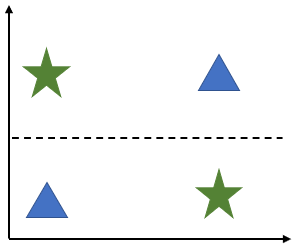
\includegraphics[scale=0.4]{media/perceptron_1}
    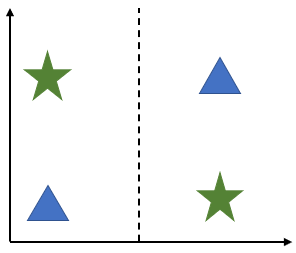
\includegraphics[scale=0.4]{media/perceptron_2}\\
    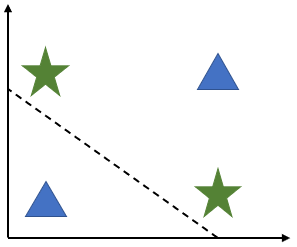
\includegraphics[scale=0.4]{media/perceptron_3}
    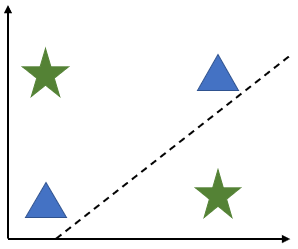
\includegraphics[scale=0.4]{media/perceptron_4}
\end{frame}

\begin{frame}{Redes Neurais Artificiais}
    \begin{itemize}
        \item MLP
            \begin{itemize}
                \justifying
                \item Solução: redes com uma ou mais camadas escondidas/intermediárias.
                \item<2-> Duas camadas intermediárias são suficientes para a aproximação de qualquer função \cite{blc00}.
            \end{itemize}
    \end{itemize}
    \centering
    \uncover<3>{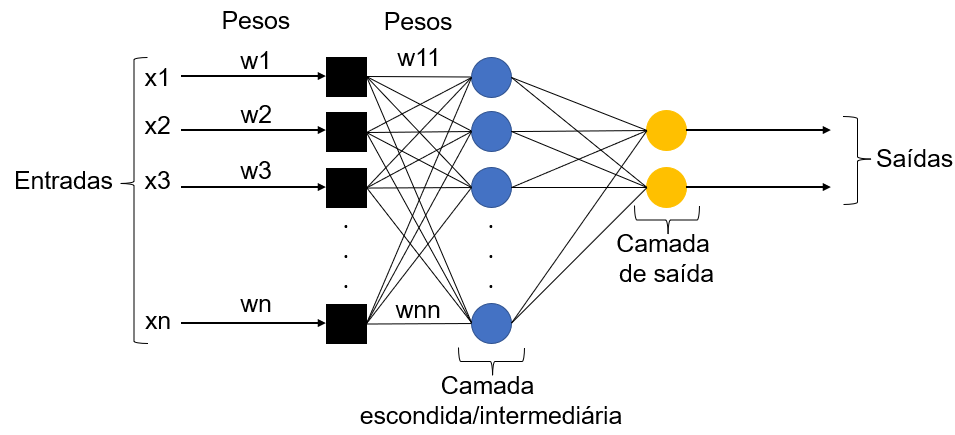
\includegraphics[width=\textwidth]{media/mlp}}
\end{frame}

\begin{frame}{Redes Neurais Artificiais}
    \begin{itemize}
        \item MLP
            \begin{itemize}
                \justifying
                \item A MLP funciona de forma semelhante ao Perceptron (pesos, função de ativação, etc.).
                \item Entretanto, fica em aberto quantas camadas e quantos neurônios em cada camada escondida são necessários/suficientes.
                \item Além disso fica também em aberto como os neurônios vão se ligar (abordagem mais comum: completamente ligados).
                \item Por fim, o aprendizado, ou seja, a atualização dos pesos se torna mais complexa (Backpropagation foi o algoritmo que "salvou" as RNAs de serem descartadas para sempre).
            \end{itemize}
    \end{itemize}
\end{frame}

\begin{frame}{Redes Neurais Artificiais}
    \begin{itemize}
        \item MLP
            \begin{itemize}
                \justifying
                \item Vídeo de MLP sendo usado para aprender o jogo do dinossauro do Chrome \cite{up19}.
            \end{itemize}
    \end{itemize}
\end{frame}

%=============================================================================
% SECTION 3
%=============================================================================
\section{Regressão Logística}

\begin{frame}{}
    \centering
    \LARGE
    Aprendizado Supervisionado\\
    \vspace{0.5cm}
    \LARGE
    Regressão\\
    \vspace{0.5cm}
    \Large
    Regressão Logística
\end{frame}

\begin{frame}{Regressão Logística}
    \begin{itemize}
        \justifying
        \item<1> Imagine um conjunto de dados contendo $N$ pontos. Cada ponto $i$ consiste de uma série de $m$ variáveis de entrada $x_{1,i}, ..., x_{m,i}$ (variáveis independentes, ou atributos) e uma saída binária $Y_{i}$ (variável dependente, ou classe), ou seja, a saída só pode assumir dois valores 0 ou 1. O objetivo da Regressão Logística é utilizar o conjunto de dados para criar um modelo preditivo para a variável de saída.
        \item<2> A função logística é uma função sigmoide:
    \end{itemize}
    \centering
    \uncover<2>{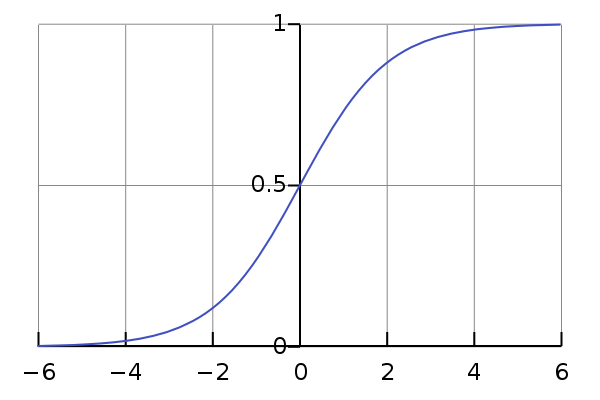
\includegraphics[scale=0.25]{media/logistic-curve}}
\end{frame}

\begin{frame}{Regressão Logística}
    \begin{itemize}
        \item Função logística:\\
        $\delta: \mathbb{R} \rightarrow (0,1)$\\
        $\delta(t) = \dfrac{\mathrm{e}^{t}}{\mathrm{e}^{t} + 1} = \dfrac{1}{1 + \mathrm{e}^{-t}}$
        \item<2-> Assumindo que $t$ é uma função linear, então $t = \beta_{0} + \beta_{1}x$\\
        Substituindo: $p(x) = \delta(t) = \dfrac{1}{1 + \mathrm{e}^{-(\beta_{0} + \beta_{1}x)}}$
    \end{itemize}
\end{frame}

\begin{frame}{Regressão Logística}
    \begin{itemize}
        \justifying
        \item Pulando toda a matemática que ainda tem depois da função apresentada, vamos ver um pequeno exemplo.\\
        \begin{exampleblock}{Exemplo}
            \begin{itemize}
                \justifying
                \item Um grupo de 20 estudantes passou de 0 a 6 horas estudando para uma prova. Os dados mostram, para cada aluno, o quanto ele estudou e se passou (1) ou não (0). Com a regressão logística, vamos ver a probabilidade de passar na prova levando em consideração o tempo de estudo.
            \end{itemize}
            \begin{table}[]
                \centering
                \tiny
                \setlength\tabcolsep{1pt}
                \begin{tabular}{l|c|c|c|c|c|c|c|c|c|c|c|c|c|c|c|c|c|c|c|c}
                    \hline
                    \textbf{Horas$(x_{k})$} & 0,5 & 0,75 & 1,00 & 1,25 & 1,50 & 1,75 & 1,75 & 2,00 & 2,25 & 2,50 & 2,75 & 3,00 & 3,25 & 3,50 & 4,00 & 4,25 & 4,50 & 4,75 & 5,00 & 5,50\\
                    \hline
                    \textbf{Resultado$(y_{k})$} & 0 & 0 & 0 & 0 & 0 & 0 & 1 & 0 & 1 & 0 & 1 & 0 & 1 & 0 & 1 & 1 & 1 & 1 & 1 & 1\\
                    \hline
                \end{tabular}
                \caption{Base de Dados}
                \label{t1}
            \end{table}
        \end{exampleblock}
    \end{itemize}
\end{frame}

\begin{frame}{Regressão Logística}
    \centering
    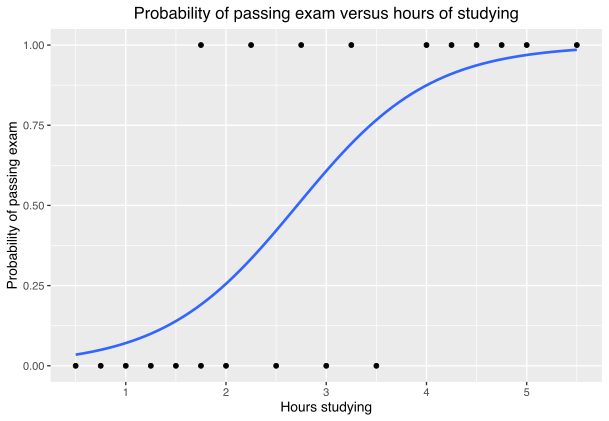
\includegraphics[width=\textwidth]{media/exam_pass_logistic_curve}
\end{frame}

%=============================================================================
% SECTION 4
%=============================================================================
\section{k-Means}

\begin{frame}{}
    \centering
    \LARGE
    Aprendizado Não Supervisionado\\
    \vspace{0.5cm}
    \LARGE
    k-Means
\end{frame}

\begin{frame}{k-Means}
    \begin{itemize}
        \justifying
        \item k-Means é um algoritmo de \textit{clusterização} (ou agrupamento).
        \item O termo significa k médias, onde k é um número inteiro qualquer.
        \item<2-> Pseudo-Algoritmo:
            \begin{enumerate}
                \item<3-> Posicione $k$ centroides aleatoriamente no espaço amostral;
                \item<4-> $\forall$ a $\in$ A $\{a \in k_{i}| dist(a,k_{i}) = min(dist(a, k))\}$;
                \item<5-> Atualize os centroides;
                \item<6> Enquanto a posição dos centroides modifica, repita os passos 2 e 3;
            \end{enumerate}
    \end{itemize}
\end{frame}

\begin{frame}{k-Means}
    \centering
    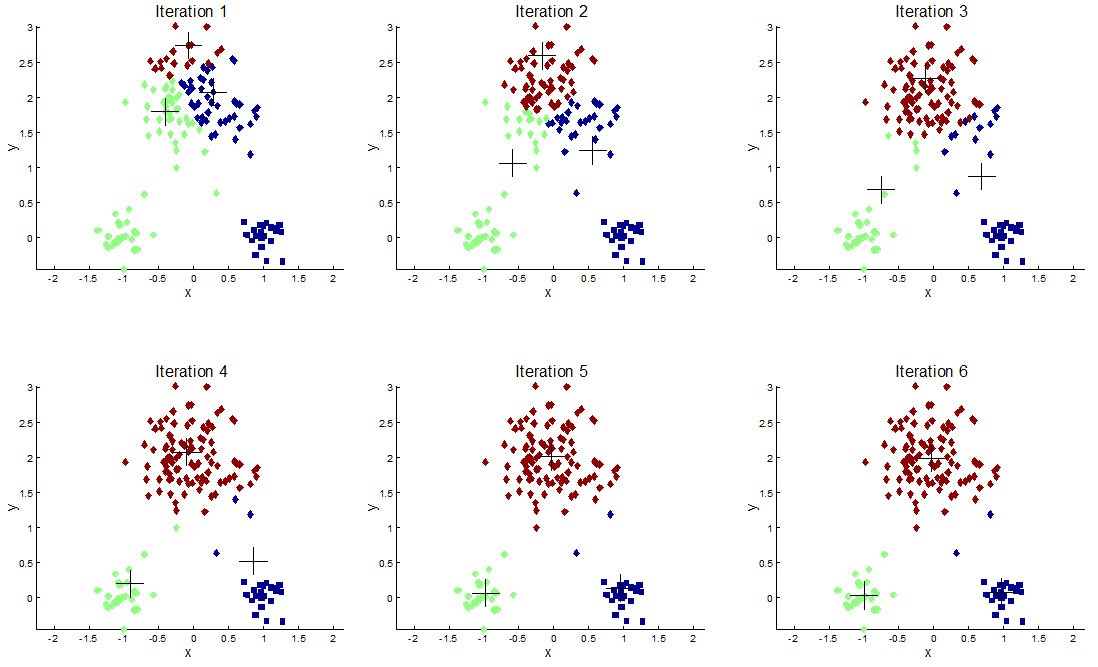
\includegraphics[width=\textwidth]{media/kmeansclustering}
\end{frame}

%=============================================================================
% SECTION FINAL
%=============================================================================
\section{FIM}

\begin{frame}{FIM}
    \centering
    \LARGE
    Finalmente terminamos!\\
    Espero que tenham gostado!\\
    \vspace{1cm}
    Obrigado pela atenção e paciência!
\end{frame}

%=============================================================================
% SECTION REFERENCES
%=============================================================================
\begin{frame}[allowframebreaks]{Referências}
    \scriptsize
    \printbibliography
\end{frame}

\end{document}













%% ---------------------------------------------------------------------------
% This presentation is separated by sections and subsections
%\section{Seção I}
%\begin{frame}{Explicações}
%    % itemize
%    Este é um template que pode ser utilizado para:
%    \begin{itemize}
%        \item Apresentação de Trabalhos Acadêmicos
%        \item Apresentação de Disciplinas
%        \item Apresentações de Teses e Dissertações
%    \end{itemize}
%
%    \vspace{0.4cm} % vertical space
%    
%    % enumeration
%    Para utilizar este template corretamente é importante que:
%    \begin{enumerate}
%        \item Tenha conhecimento mínimo sobre LaTeX
%        \item Ler os comentários no template (explicações)
%        \item Ler o README.md (documentação)
%    \end{enumerate}
%
%    \vspace{0.2cm}

%    \example{Este é um texto de exemplo!} \emph{Texto de Ênfase!}
%\end{frame}

%% ---------------------------------------------------------------------------
%\subsection{Subseção I}
%\begin{frame}{Criando Blocos}
%    % Blocks styles
%    \begin{block}{Bloco Padrão}
%        Texto do corpo do bloco.
%    \end{block}

%    \begin{alertblock}{Bloco de Alerta}
%        Texto do corpo do bloco.
%    \end{alertblock}
%
%    \begin{exampleblock}{Bloco de Exemplo}
%        Texto do corpo do bloco.
%    \end{exampleblock}   
%\end{frame}

%% ---------------------------------------------------------------------------
%\subsection{Subseção II}
%\begin{frame}{Criando Caixas}
%    \successbox{testando o success box}
%
%    \pause
%
%    \alertbox{testando o alert box}
%
%    \pause
%
%    \simplebox{testando o simple box}
%\end{frame}

%% ---------------------------------------------------------------------------
%\subsection{Subseção III}
%\begin{frame}{Criando Algoritmos (Pseudocódigo)}
%    \begin{algorithm}[H]
%        \SetAlgoLined
%        \LinesNumbered
%        \SetKwInOut{Input}{input}
%        \SetKwInOut{Output}{output}
%        \Input{x: float, y: float}
%        \Output{r: float}
%        \While{True}{
%          r = x + y\;
%          \eIf{r >= 30}{
%           ``O valor de $r$ é maior ou iqual a 10.''\;
%           break\;
%           }{
%           ``O valor de $r$ = '', r\;
%          }
%         } 
%         \caption{Algorithm Example}
%    \end{algorithm}
%\end{frame}

%% ---------------------------------------------------------------------------

%\begin{frame}{Inserindo Algoritmos}
%    \lstset{language=Python}
%    \lstinputlisting[language=Python]{code/main.py}
%\end{frame}

%% ---------------------------------------------------------------------------
%\begin{frame}{Inserindo Algoritmos}
%    \lstinputlisting[language=C]{code/source.c}
%\end{frame}

%% ---------------------------------------------------------------------------
%\begin{frame}{Inserindo Algoritmos}
%    \lstinputlisting[language=Java]{code/helloworld.java}
%\end{frame}

%% ---------------------------------------------------------------------------
%\begin{frame}{Inserindo Algoritmos}
%    \lstinputlisting[language=HTML]{code/index.html}
%\end{frame}

%% ---------------------------------------------------------------------------
% This frame show an example to insert multicolumns
%\section{Multicolunas}
%\begin{frame}{Seção II - Multicolunas}
%    \begin{columns}{}
%        \begin{column}{0.5\textwidth}
%            \justify
%            É possível colocar mais de uma coluna utilizando os comandos de $\backslash$begin\{column\}\{\} e $\backslash$end\{column\}
%        \end{column}
%        \begin{column}{0.5\textwidth}
%            \justify
%            Porém, o espaçamento deve ser proporcional entre as colunas para que estas colunas não entrem em coflito. O espaçamento é dado pelo segundo argumento do $\backslash$begin.
%        \end{column}
%    \end{columns}    
%\end{frame}

%% ---------------------------------------------------------------------------
% This frame show an example to insert figures
%\section{Imagens}
%\begin{frame}{Seção III - Figures}
%    \begin{figure}
%        \centering
%        \caption{Emblema da UFC.}
%        
\includegraphics[scale=0.3]{libs/emblemufc.pdf}
%        \source{Obtido pelo site oficial da UFC \cite{siteufc} \cite{einstein}}
%        \label{fig:ufc_emblem}
%    \end{figure}
%\end{frame}

%% ---------------------------------------------------------------------------
% Reference frames
%\begin{frame}[allowframebreaks]
%    \frametitle{Referências}
%    \printbibliography
%\end{frame}

%% ---------------------------------------------------------------------------
% Final frame
%\begin{frame}{}
%    \centering
%    \huge{\textbf{\example{Obrigado(a) pela Atenção!}}}
%    
%    \vspace{1cm}
%    
%    \Large{\textbf{Contato:}}
%    \newline
%    \vspace*{0.5cm}
%    \large{\email{usuario@dominio}}
%\end{frame}